\documentclass[a4]{article}

\usepackage[left=3cm,right=3cm,top=2cm,bottom=2cm]{geometry} 

\usepackage[utf8]{inputenc}   % otra alternativa para los caracteres acentuados y la "ñ"
\usepackage[           spanish % para poder usar el español
                      ,es-tabla % para los captions de las tablas
                       ]{babel}   
\decimalpoint %para usar el punto decimal en vez de coma para los números con decimales

\usepackage[bookmarks=true,
            bookmarksnumbered=false, % true means bookmarks in 
                                     % left window are numbered              
            bookmarksopen=false,     % true means only level 1
                                     % are displayed.
            colorlinks=true,
            linkcolor=blue,
            urlcolor=cyan]{hyperref}
            
\usepackage[T1]{fontenc}
\usepackage{lmodern}

\usepackage{parskip}
\usepackage{xcolor}

\usepackage{amsmath,amssymb,amsthm}

\usepackage{caption}

\usepackage{listings}
\lstset
{ %Formatting for code in appendix
  language=C++, % choose the language of the code
  basicstyle=\fontfamily{pcr}\selectfont\footnotesize\color{black},
  keywordstyle=\color{darkorange}\bfseries, % style for keywords
  numbers=left, % where to put the line-numbers
  numberstyle=\tiny, % the size of the fonts that are used for the line-numbers     
  backgroundcolor=\color{white},
  showspaces=false, % show spaces adding particular underscores
  showstringspaces=false, % underline spaces within strings
  showtabs=false, % show tabs within strings adding particular underscores
  tabsize=2, % sets default tabsize to 2 spaces
  captionpos=b, % sets the caption-position to bottom
  breaklines=true, % sets automatic line breaking
  breakatwhitespace=false, 
}

\usepackage{enumerate}% paquete para poder personalizar fácilmente la apariencia de las listas enumerativas

\usepackage{graphicx} % figuras
\usepackage{subfigure} % subfiguras

\definecolor{darkorange}{rgb}{0.4,0,0.8}
	
\usepackage{float} % para controlar la situación de los entornos flotantes

\restylefloat{figure}
\restylefloat{table} 

\newcommand{\HRule}{\rule{\linewidth}{0.5mm}}

\author{David Cabezas Berrido \\ Patricia Córdoba Hidalgo \\ Emilio José Hoyo Medina \\ Inmaculada Marín Carballo}
\date{\vspace{1mm} \today}

\title{\huge Algoritmos Backtracking y B\&B: \\Viajante de Comercio \HRule\vspace{-4mm} }

\setcounter{section}{-1}

\begin{document}
\maketitle
\vspace{5mm}
\tableofcontents
\newpage

\section{Problema}
\subsection{Viajante de Comercio}
El problema del viajante de comercio (TSP, por Traveling Salesman Problem): dado un conjunto de ciudades y una matriz con las distancias entre todas ellas, un viajante debe recorrer todas las ciudades exactamente una vez, regresando al punto de partida, de forma tal que la distancia recorrida sea mínima.


\section{Clase TSP}
Hemos decicido crear una clase que albergue nuestro mapa de ciudades y que realice todas las funciones que consideramos oportunas para que el código sea lo más sencillo posible:

\subsection{Código}
\begin{lstlisting}
class TSP{

private:
  int n;
  vector<vector<int>> map;

public:

  vector<double> xCords, yCords;

  TSP(string file){

    ifstream f(file);
    
    string trash;
    f >> trash;
    f >> n;

    int i, j;
    double c;
    //Leo los datos del fichero
    for(j = 0; j < n; j++){
      f >> i;
      f >> c;
      xCords.push_back(c);
      f >> c;
      yCords.push_back(c);
    }

    f.close();

    int distance;
    vector<vector<int>> aux(n);
    
    for(i = 1; i < n; i++){
      for(j = 0; j < i; j++){
	distance = (int) rint(sqrt(pow(xCords[i]-xCords[j],2) + pow((yCords[i]-yCords[j]),2)));
	aux[i].push_back(distance);
      }
    }
    map = aux;
  }

  int getN() const{
    return n;
  }

  void printMap() const{
    int i, j;

    for(i = 0; i < n; i++){
      for(j = 0; j < i; j++){
	cout << map[i][j] << "\t";
      }
      cout << endl;
    }
  }

  int getDistance(int i, int j) const{
    if(0 <= i && i < n && 0 <= j && j < n)
      return map[max(i,j)][min(i,j)];

    return INT_MAX; // Para evitar considerar la distancia de una ciudad a si misma
  }

  int totalWeight(vector<int> solution) const{
    assert(solution.size() == n);
    int weight = 0;
    for(int i = 0; i < n; i++)
      weight += getDistance(i,(i-1+n)%n);

    return weight;
  }

  // Devuelve la distancia de city a su ciudad mas cercana
  int bestDistance(int city) const{
    int minD = getDistance(city,0);
    
    for(int j = 1; j < n; j++)
      if(getDistance(city,j) < minD)
	minD = getDistance(city,j);

    return minD;
  }

  int weightBound(const vector<int> &visited, int currentWeight) const{
    int bound = currentWeight;

    for(int i = 1; i < n; i++)
      if(find(visited.begin(),visited.end(),i)==visited.end())
	bound += bestDistance(i);

    return bound;
  }
};
\end{lstlisting}

\section{Backtracking}
Aplicaremos la técnica de \textbf{Backtracking} para encontrar la
solución óptima al problema. \\
Nuestro algoritmo de Bactracking recorre todas las posibilidades en nuestro árbol. Pero se diferencia del algortimo de ''fuerza bruta'' en que una vez encuentra que la posibilidad estudiada supera la cota que hemos determinado la podará. Esta cota se calcula gracias a una función que determina un arco mínimo, concepto estudiado en teoría.

\subsection{Código}
Fuera de la clase TSP declaramos la función recursiva que llevará acabo nuestro algoritmo:
\begin{lstlisting}
void backtracking(const TSP& tsp, const vector<int> &visited, vector<int> &bestSol, int currentWeight, int& minimumWeight){

  if(visited.size() == tsp.getN()){
    currentWeight += tsp.getDistance(visited.back(),visited.front());
    if(currentWeight < minimumWeight){
      minimumWeight = currentWeight;
      bestSol = visited;
    }
    return;
  }

  if(tsp.weightBound(visited, currentWeight) >= minimumWeight)
    return;

  int weight;
  vector<int> aux;

  for(int i = 1; i < tsp.getN(); i++){
    weight = currentWeight;
    aux = visited;
    if(find(visited.begin(),visited.end(),i)==visited.end()){
      aux.push_back(i);
      weight += tsp.getDistance(i,visited.back());
      backtracking(tsp, aux, bestSol, weight, minimumWeight);
    }
  }
}
\end{lstlisting}

Donde los datos de entrada son:
\begin{itemize}
\item tsp: Un objeto de la clase TSP con los datos de las ciudades.
\item visited: Vector con las ciudades ya visitadas
\item bestSol: Vector con la mejor solución encontrada
\item currentWeight: Peso que tiene el camino recorrido hasta el momento
\item minimumWeight: Peso mínimo encontrado en una solución
\end{itemize}

\section{Branch and Bound}

Ahora resolveremos el problema con un algoritmo de \textbf{Branch and Bound}. La diferencia con Backtracking es que en este último se hace en
profundidad. Empiezo por un nodo y sigo para abajo. Cuando termino un recorrido es porque, o bien he obtenido una solución, o bien he tenido que podar la rama. Siempre que cojo un nodo expando sólo uno.
Sin embargo en Branch and Bound cuando expando un nodo, expando a la vez todos sus hijos. De entre todos los nodos vivos, me quedo con el que tenga la estimación más prometedora, y expando todos los hijos de este. En función de la estimación voy expandiendo los nodos.

\subsection{Código}

\begin{lstlisting}
void BandB(const TSP &tsp, multiset<node> &alive_nodes, vector<int> &bestSol, int &minimumWeight, int &maxsize, int &expanded, int &pruned){

  //Actualizamos la variable maxsize
  if(alive_nodes.size() > maxsize)
    maxsize = alive_nodes.size();

  //Si nos quedamos sin nodos vivos, salimos de la funcion
  if(alive_nodes.empty()) return;

  //Tomamos el nodo mas prometedor
  node n = *alive_nodes.begin();

  alive_nodes.erase(alive_nodes.begin());

  //Si su cota es mayor que la minima cota encontrada, ya el resto tendran cota peor -> salimos de la funcion
  if(n.bound >= minimumWeight)
    return;

  //Si encontramos una solucion, vemos si es optima
  if(n.visited.size() == tsp.getN()){
 
    n.currentWeight += tsp.getDistance(n.visited.front(), n.visited.back());

    if(n.currentWeight < minimumWeight){
      minimumWeight = n.currentWeight;
      bestSol = n.visited;
      pruned = prune(alive_nodes,minimumWeight);
    }
    //Seguimos buscando soluciones
    BandB(tsp, alive_nodes, bestSol, minimumWeight, maxsize, expanded, pruned);
  }
  //Si no hemos encontrado solucion, expandimos
  else { 
    node aux;

    expanded++;
  
    for(int i = 1; i < tsp.getN(); i++){
      if(find(n.visited.begin(), n.visited.end(), i) == n.visited.end()){
	aux = n;
	aux.visited.push_back(i);
	aux.currentWeight += tsp.getDistance(i, n.visited.back());
	aux.bound = tsp.weightBound(aux.visited, aux.currentWeight);
	alive_nodes.insert(aux);
      }
    }

    BandB(tsp, alive_nodes, bestSol, minimumWeight, maxsize, expanded, pruned);
  }
}

\end{lstlisting}

Donde los datos de entrada son:
\begin{itemize}
\item tsp: Un objeto de la clase TSP con los datos de las ciudades.
\item alive\_nodes: Multiset con los nodos vivos del árbol
\item bestSol: Vector con la mejor solución encontrada
\item minimumWeight: Peso mínimo encontrado en una solución
\item maxsize: Tamaño máximo del multiset
\item expanded: Veces que hemos expandido un nodo
\item pruned: Veces que hemos podado un nodo
\end{itemize}

\section{Eficiencia}

La eficiencia teórica de ambos algoritmos, backtracking y branch\&bound, es $O((n-1)!)$. Esto se debe a que hay que recorrer todo el árbol para buscar la mejor solución entre todas las posibles, que son las permutaciones de $n-1$ elementos. Son $n-1$ porque la primera ciudad siempre es la primera del fichero pasado.
Sin embargo, debido a las funciones que calculan las cotas, hay partes del árbol que se podan, luego empíricamente la eficiencia es menor.

\section{Resultados Empíricos}

Hemos adaptado nuestra selección de tamaños para que fueran fáciles de utilizar con los tres algortimos (que los resultados fueran ciertamente diferenciables y la ejecución no se prolongara demasiado). En esta tabla exponemos los tiempos de ejecución para cada tamaño de 4 a 15, por cada algoritmo:

\begin{figure}[H]
  \centering
  \label{tab:tiempos}
  \begin{tabular}{| c | c | c | c |}
    \hline
    \multicolumn{1}{|c|}{$\textbf{n}$}& \textbf{Backtracking}&
    \textbf{Branch and Bound}& \textbf{Greedy} \\ \hline
     4 & 6e-06	   & 5.7e-05  & 0.00010  \\ 
     5 & 1.2e-05   & 0.00022  & 0.00040  \\ 
     6 & 1.8e-05   & 0.00094  & 0.00183  \\ 
     7 & 2.7e-05   & 0.00244  & 0.00423  \\ 
     8 & 3.5e-05   & 0.00131  & 0.00278  \\ 
     9 & 5e-05	   & 0.00593  & 0.00623  \\ 
    10 & 6.7e-05   & 0.35094  & 0.09896  \\ 
    11 & 8.8e-05   & 0.41862  & 0.98615  \\ 
    12 & 0.000106  & 0.60728  & 1.76516  \\
    13 & 0.000131  & 1.17463  & 2.64651  \\
    14 & 0.000166  & 1.52913  & 3.60603  \\
    15 & 0.000202  & 3.14079  & 6.45577  \\ \hline
  \end{tabular}
\end{figure}

\subsection{Gráficas}

\begin{figure}[H]
  \centering
  \subfigure[Backtracking]{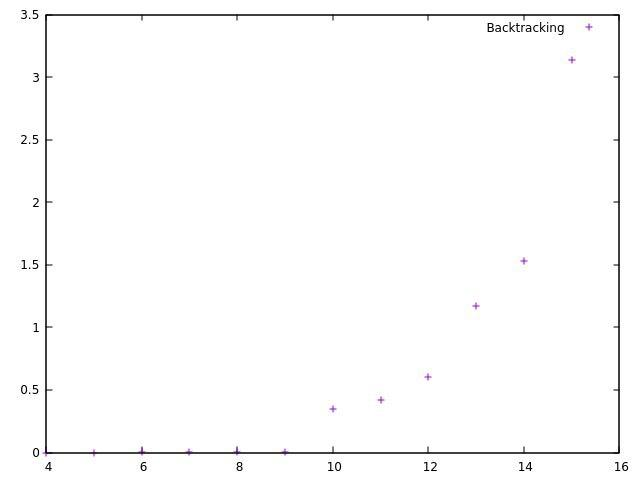
\includegraphics[width=65mm]{graficas/tiempos/backtracking}}
  \subfigure[Branch and Bound]{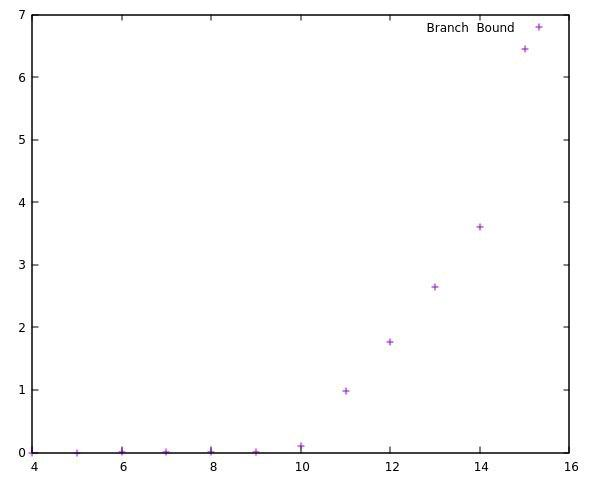
\includegraphics[width=65mm]{graficas/tiempos/B&B}}
  \subfigure[Branch and Bound]{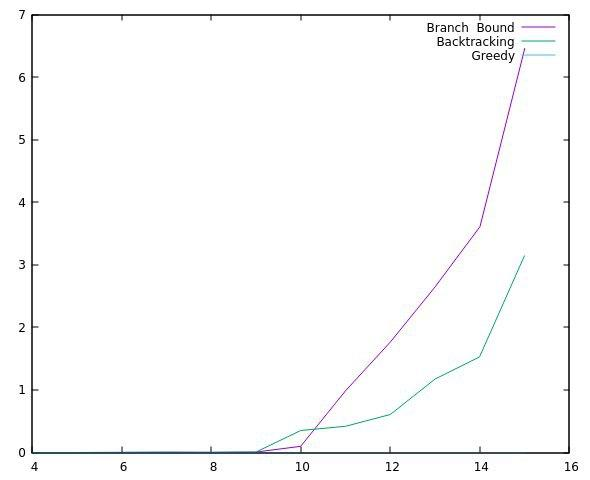
\includegraphics[width=80mm]{graficas/tiempos/comparacion}}
\end{figure}

\section{Recorridos}
Los recorridos dados por los algoritmos son:

\subsection{a4}
\setcounter{subfigure}{0}

Branch and Bound:
\begin{itemize}
\item Nodos expandidos: 7
\item Podas: 2
\item Nº máximo de nodos vivos simultáneamente: 4 
\end{itemize}

\begin{figure}[H]
  \centering
  \subfigure[Greedy. Peso = 55]{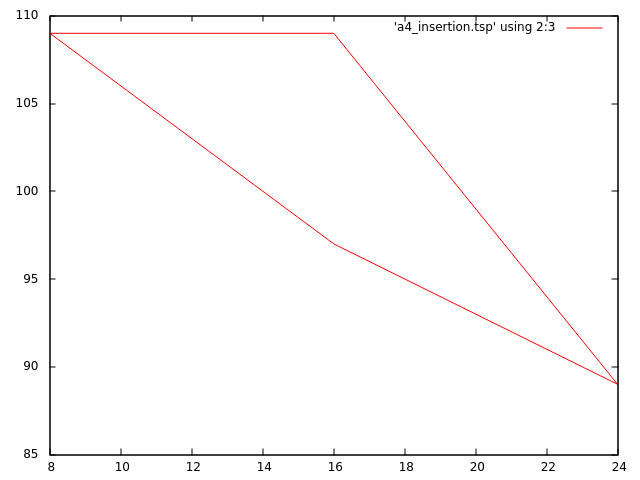
\includegraphics[width=70mm]{graficas/Greedy/a4}}
  \subfigure[Backtracking. Peso = 55]{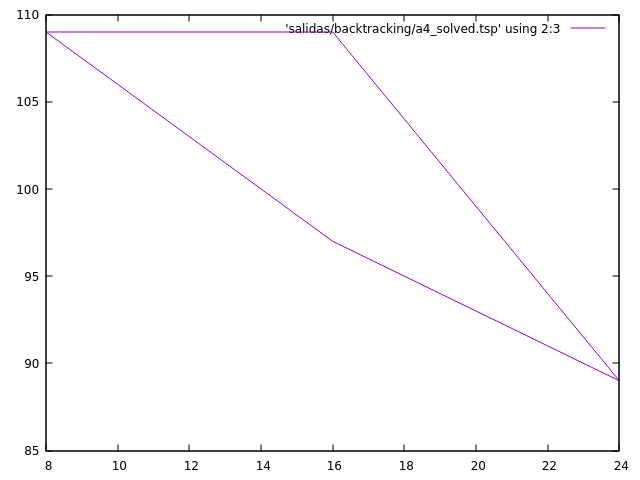
\includegraphics[width=70mm]{graficas/Backtracking/a4}}
  \subfigure[Branch and Bound. Peso = 55]{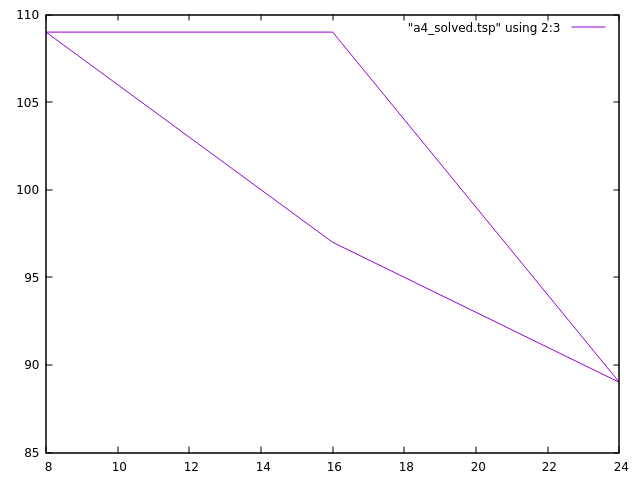
\includegraphics[width=70mm]{graficas/B&B/a4}}
\end{figure}

\newpage

\subsection{att5}
\setcounter{subfigure}{0}

Branch and Bound:
\begin{itemize}
\item Nodos expandidos: 23
\item Podas: 12
\item Nº máximo de nodos vivos simultáneamente: 15
\end{itemize}

\begin{figure}[H]
  \centering
  \subfigure[Greedy. Peso = 10060]{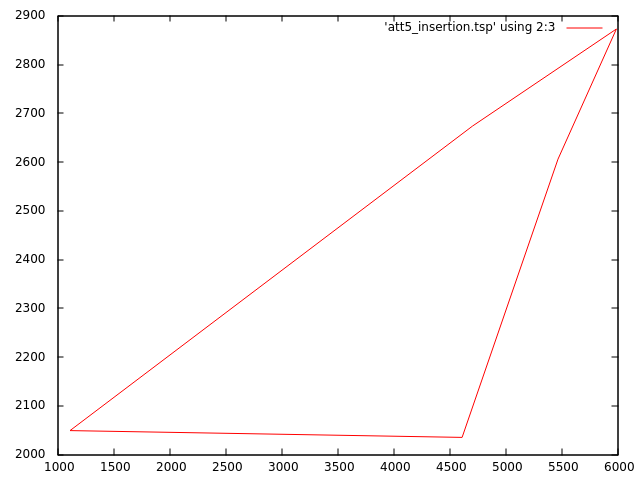
\includegraphics[width=70mm]{graficas/Greedy/att5}}
\subfigure[Backtracking. Peso = 10060]{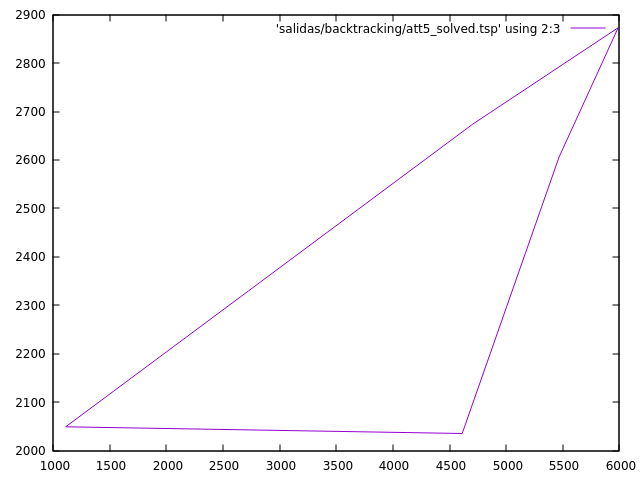
\includegraphics[width=70mm]{graficas/Backtracking/att5}}
\subfigure[Branch and Bound. Peso = 10060]{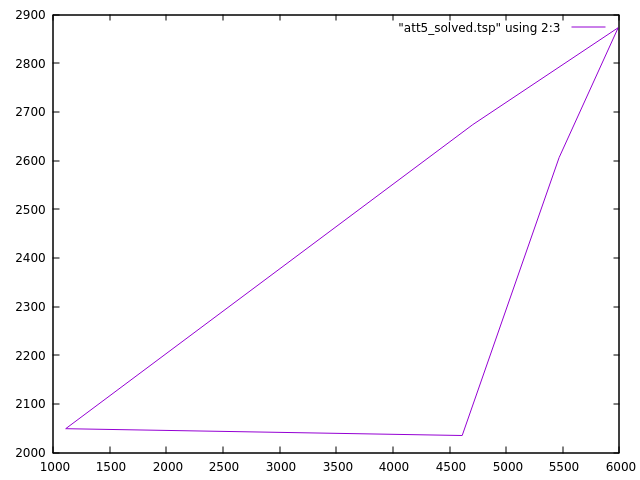
\includegraphics[width=70mm]{graficas/B&B/att5}}
\end{figure}

\newpage

\subsection{bayg6}
\setcounter{subfigure}{0}

Branch and Bound:
\begin{itemize}
\item Nodos expandidos: 77
\item Podas: 78
\item Nº máximo de nodos vivos simultáneamente: 60
\end{itemize}

\begin{figure}[H]
  \centering
  \subfigure[Greedy. Peso = 4244]{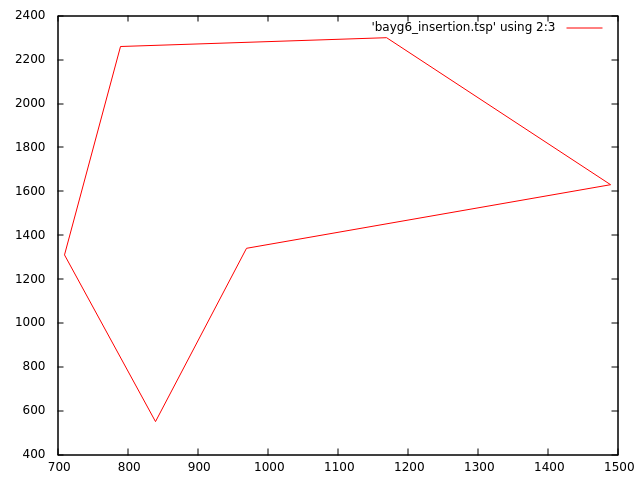
\includegraphics[width=70mm]{graficas/Greedy/bayg6}}
  \subfigure[Backtracking. Peso = 4244]{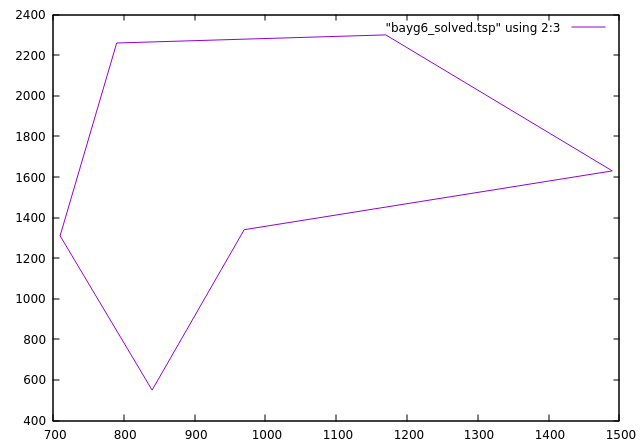
\includegraphics[width=70mm]{graficas/Backtracking/bayg6}}
  \subfigure[Branch and Bound. Peso = 4244]{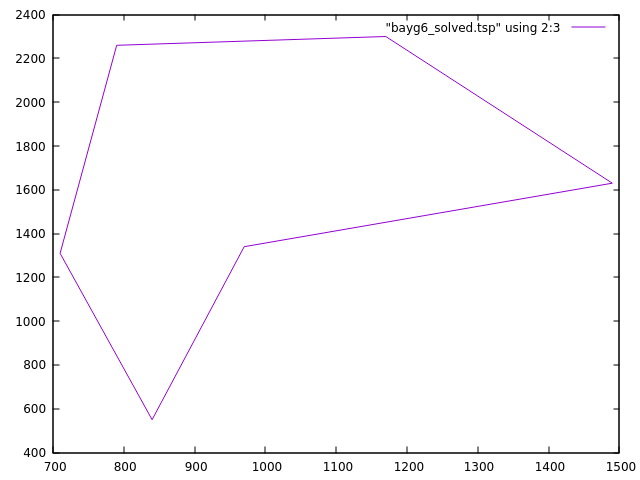
\includegraphics[width=70mm]{graficas/B&B/bayg6}}
\end{figure}

\newpage

\subsection{berlin7}
\setcounter{subfigure}{0}

Branch and Bound:
\begin{itemize}
\item Nodos expandidos: 233
\item Podas: 269
\item Nº máximo de nodos vivos simultáneamente: 249
\end{itemize}

\begin{figure}[H]
  \centering
  \subfigure[Greedy. Peso = 2218]{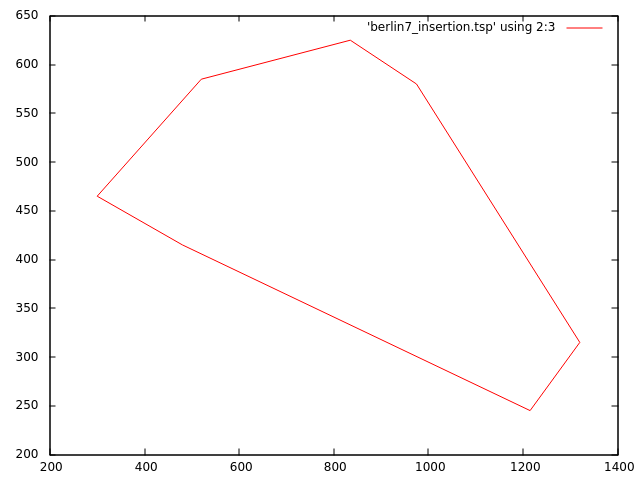
\includegraphics[width=70mm]{graficas/Greedy/berlin7}}
  \subfigure[Backtracking. Peso = 2218]{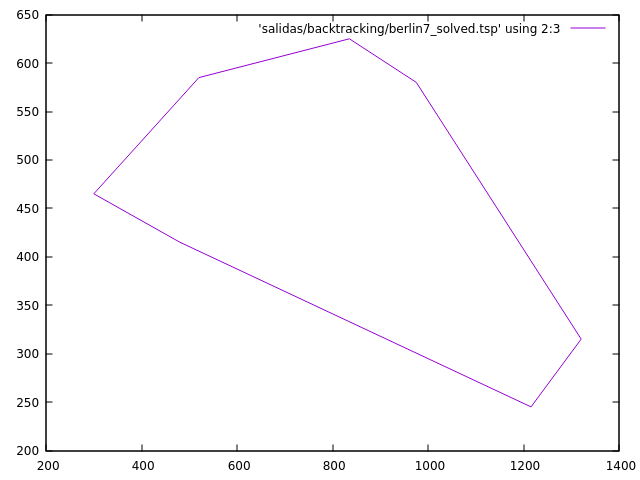
\includegraphics[width=70mm]{graficas/Backtracking/berlin7}}
  \subfigure[Branch and Bound. Peso = 2218]{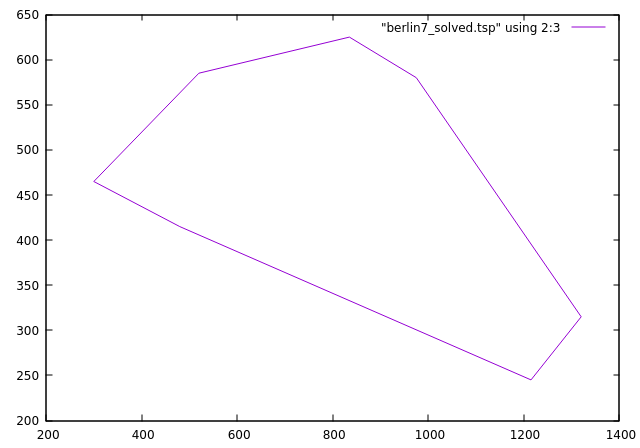
\includegraphics[width=70mm]{graficas/B&B/berlin7}}
\end{figure}

\newpage

\subsection{eil8}
\setcounter{subfigure}{0}

Branch and Bound:
\begin{itemize}
\item Nodos expandidos: 189
\item Podas: 410
\item Nº máximo de nodos vivos simultáneamente: 316
\end{itemize}

\begin{figure}[H]
  \centering
  \subfigure[Greedy. Peso = 166]{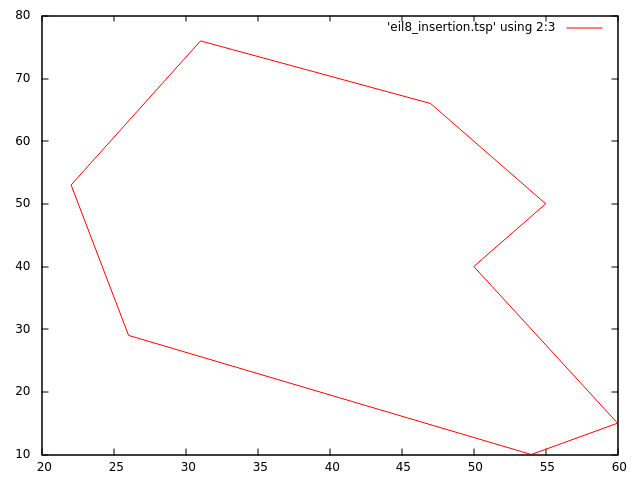
\includegraphics[width=70mm]{graficas/Greedy/eil8}}
  \subfigure[Backtracking. Peso = 166]{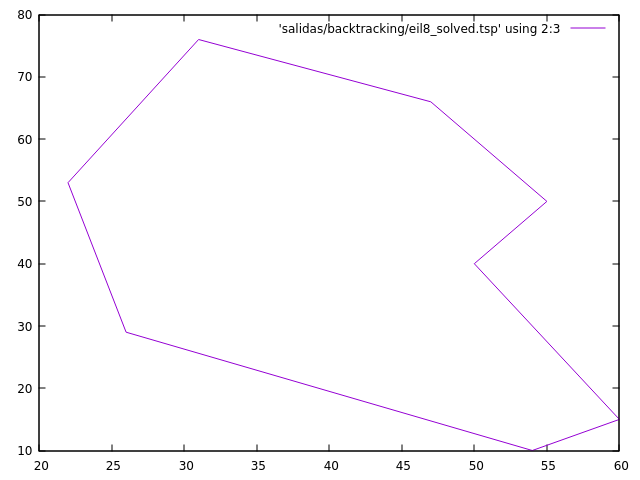
\includegraphics[width=70mm]{graficas/Backtracking/eil8}}
  \subfigure[Branch and Bound. Peso = 166]{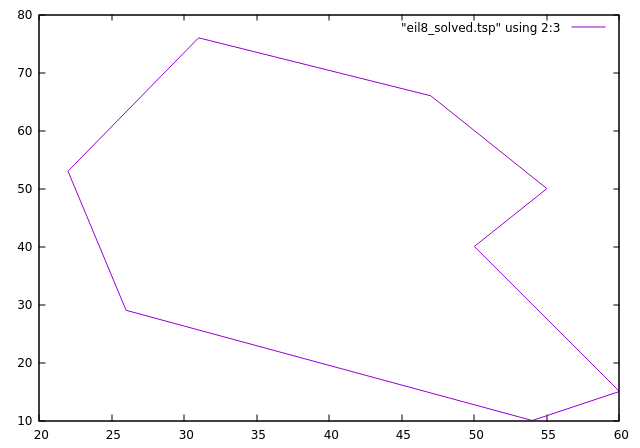
\includegraphics[width=70mm]{graficas/B&B/eil8}}
\end{figure}

\newpage

\subsection{eil9}
\setcounter{subfigure}{0}

Branch and Bound:
\begin{itemize}
\item Nodos expandidos: 367
\item Podas: 784
\item Nº máximo de nodos vivos simultáneamente: 375
\end{itemize}

\begin{figure}[H]
  \centering
  \subfigure[Greedy. Peso = 151]{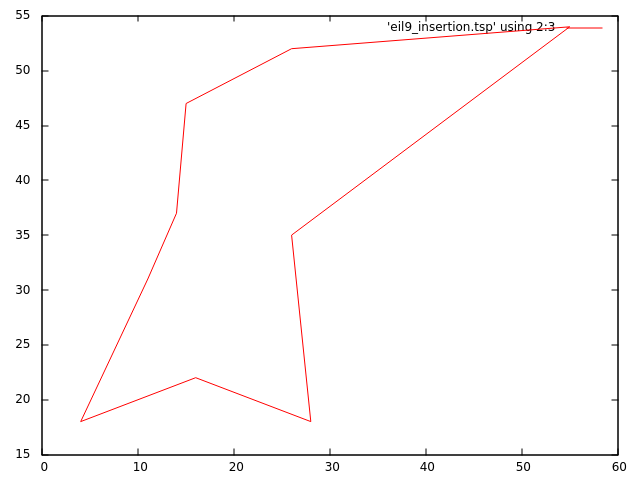
\includegraphics[width=70mm]{graficas/Greedy/eil9}}
  \subfigure[Backtracking. Peso = 151]{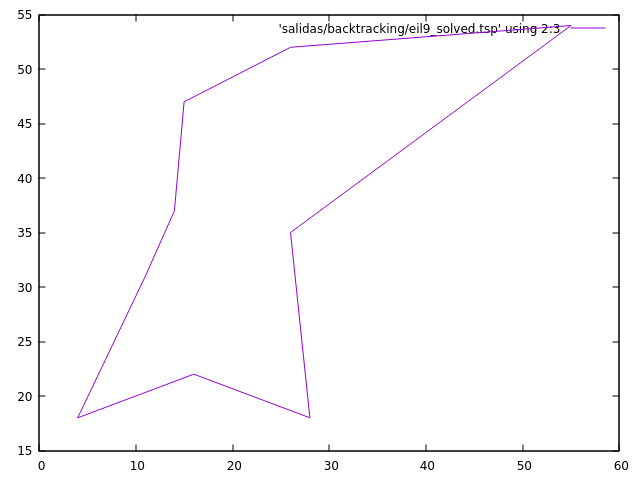
\includegraphics[width=70mm]{graficas/Backtracking/eil9}}
  \subfigure[Branch and Bound. Peso = 151]{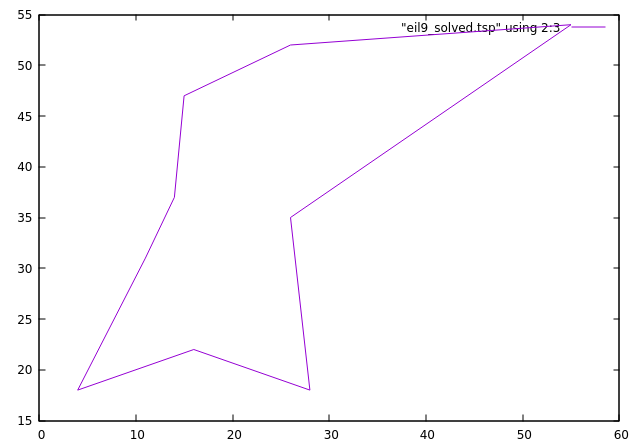
\includegraphics[width=70mm]{graficas/B&B/eil9}}
\end{figure}

\newpage

\subsection{gr10}
\setcounter{subfigure}{0}

Branch and Bound:
\begin{itemize}
\item Nodos expandidos: 69972
\item Podas: 74072
\item Nº máximo de nodos vivos simultáneamente: 70629
\end{itemize}

\begin{figure}[H]
  \centering
  \subfigure[Greedy. Peso = 129]{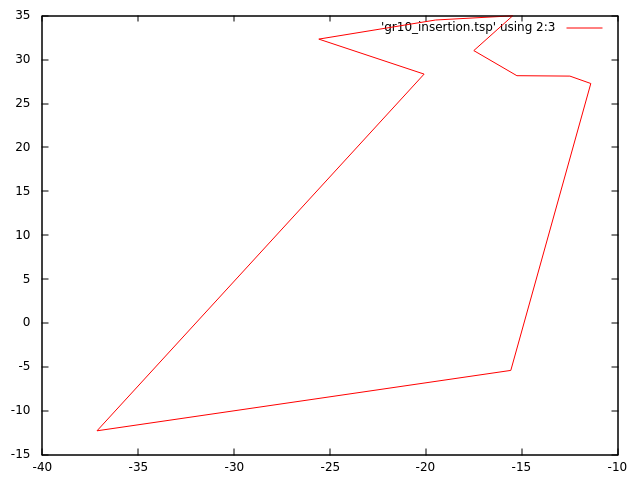
\includegraphics[width=70mm]{graficas/Greedy/gr10}}
  \subfigure[Backtracking. Peso = 129]{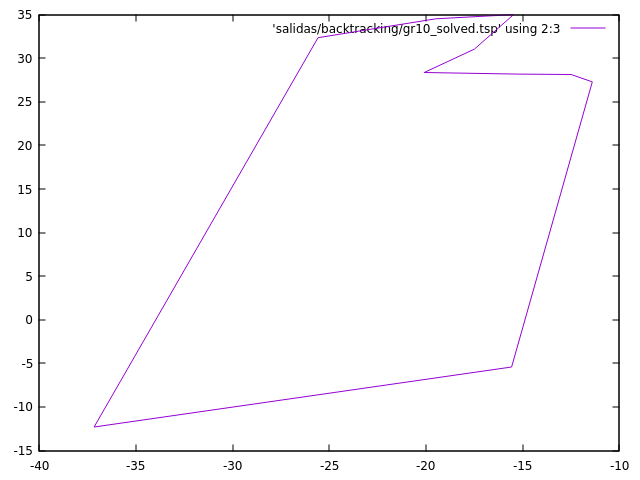
\includegraphics[width=70mm]{graficas/Backtracking/gr10}}
  \subfigure[Branch and Bound. Peso = 129]{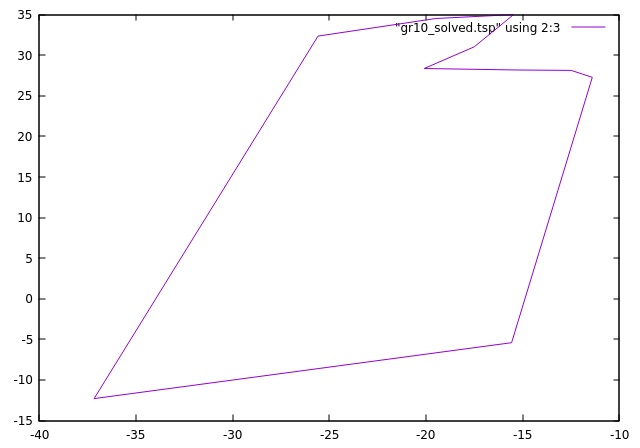
\includegraphics[width=70mm]{graficas/B&B/gr10}}
\end{figure}

\newpage

\subsection{gr11}
\setcounter{subfigure}{0}

Branch and Bound:
\begin{itemize}
\item Nodos expandidos: 121162
\item Podas: 245564
\item Nº máximo de nodos vivos simultáneamente: 162699
\end{itemize}

\begin{figure}[H]
  \centering
  \subfigure[Greedy. Peso = 99]{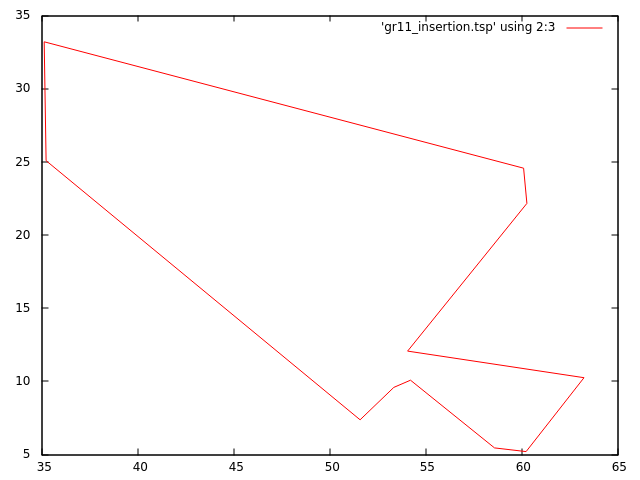
\includegraphics[width=70mm]{graficas/Greedy/gr11}}
  \subfigure[Backtracking. Peso = 92]{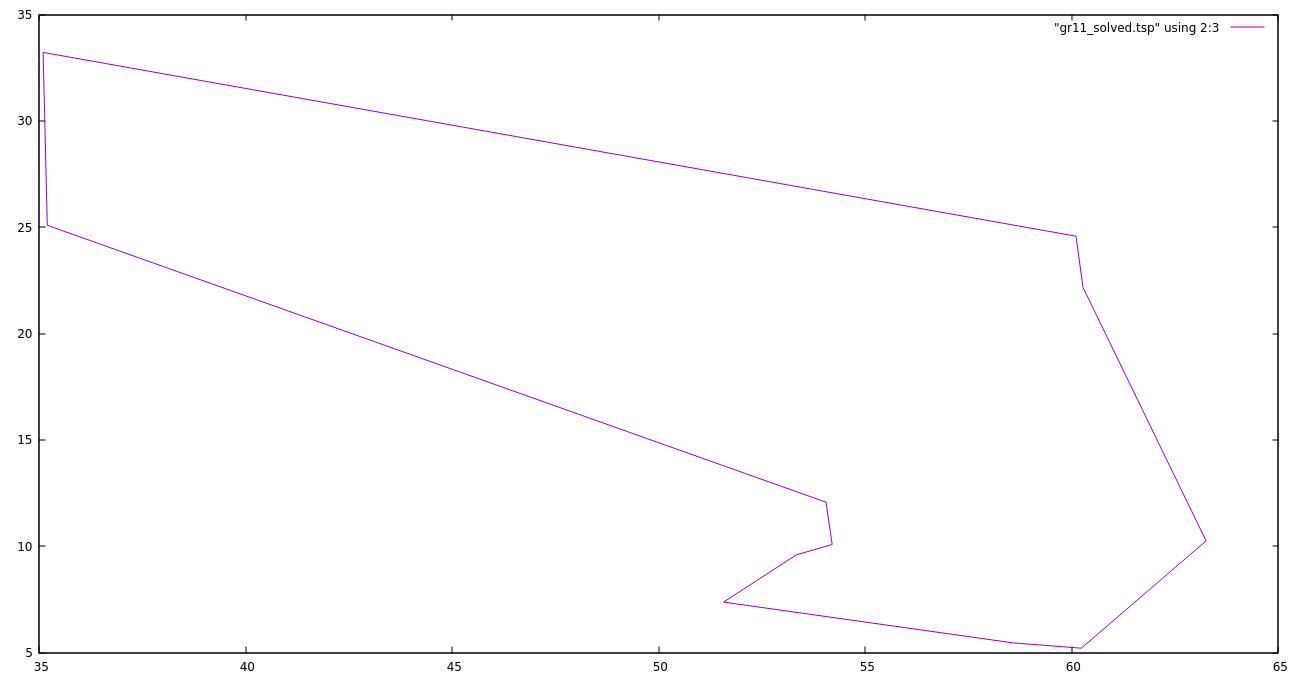
\includegraphics[width=70mm]{graficas/Backtracking/gr11}}
  \subfigure[Branch and Bound. Peso = 92]{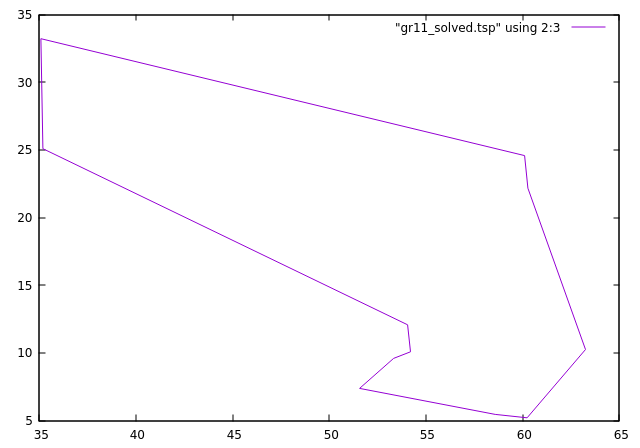
\includegraphics[width=70mm]{graficas/B&B/gr11}}
\end{figure}

\newpage

\subsection{kroD12}
\setcounter{subfigure}{0}

Branch and Bound:
\begin{itemize}
\item Nodos expandidos: 32017
\item Podas: 103296
\item Nº máximo de nodos vivos simultáneamente: 79572
\end{itemize}

\begin{figure}[H]
  \centering
  \subfigure[Greedy. Peso = 10656]{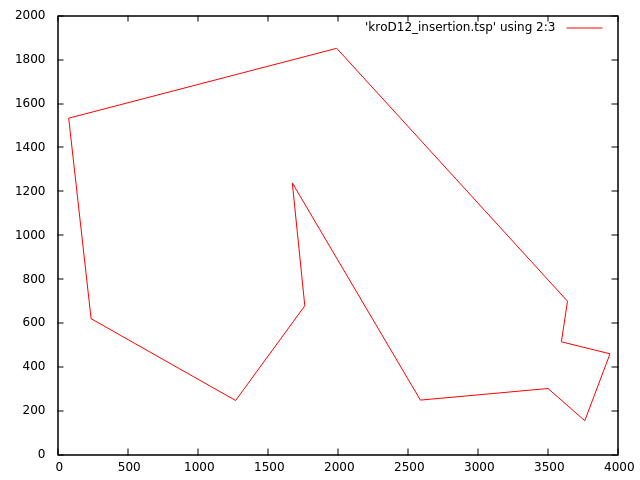
\includegraphics[width=70mm]{graficas/Greedy/kroD12}}
  \subfigure[Backtracking. Peso = 10047]{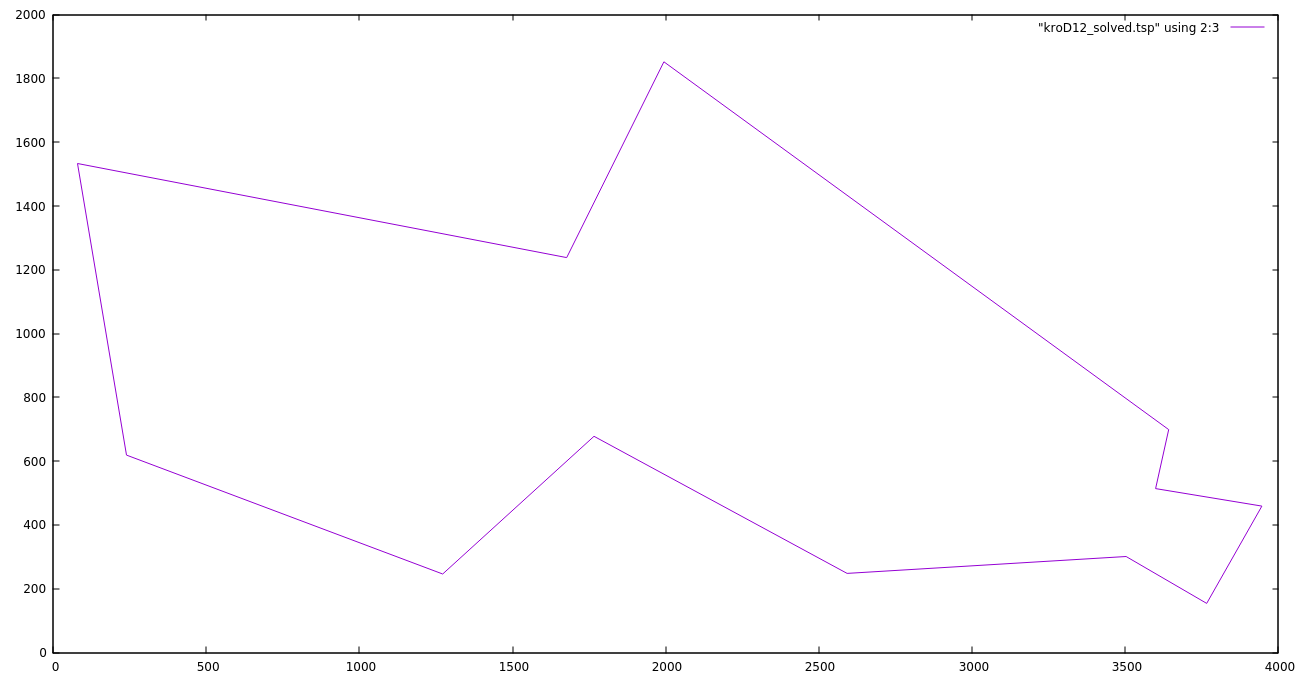
\includegraphics[width=70mm]{graficas/Backtracking/kroD12}}
  \subfigure[Branch and Bound. Peso = 10047]{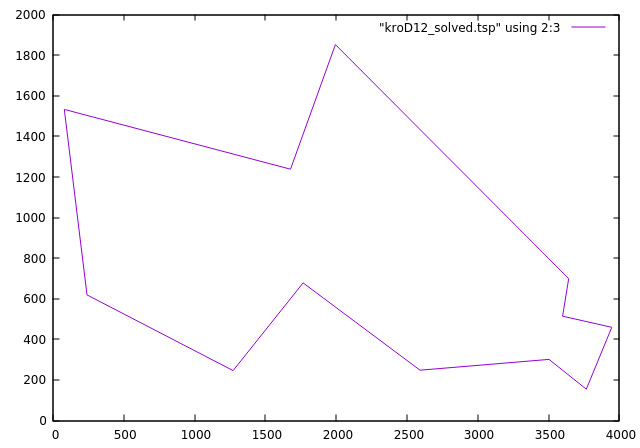
\includegraphics[width=70mm]{graficas/B&B/kroD12}}
\end{figure}

\newpage

\subsection{pcb13}
\setcounter{subfigure}{0}

Branch and Bound:
\begin{itemize}
\item Nodos expandidos: 2197231
\item Podas: 5630312
\item Nº máximo de nodos vivos simultáneamente: 5630313
\end{itemize}

\begin{figure}[H]
  \centering
  \subfigure[Greedy. Peso = 8351]{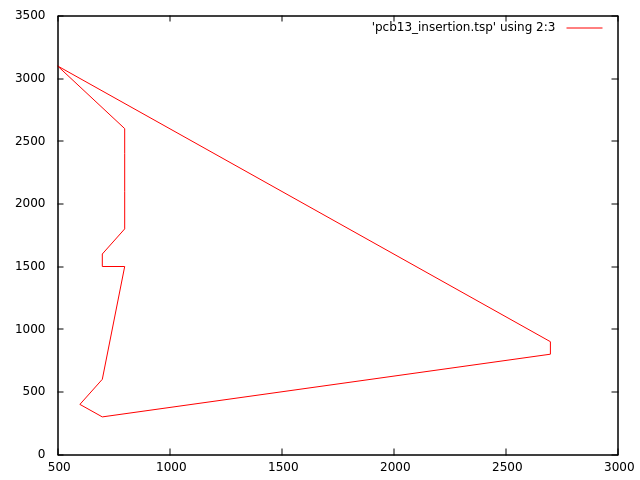
\includegraphics[width=70mm]{graficas/Greedy/pcb13}}
  \subfigure[Backtracking. Peso = 8351]{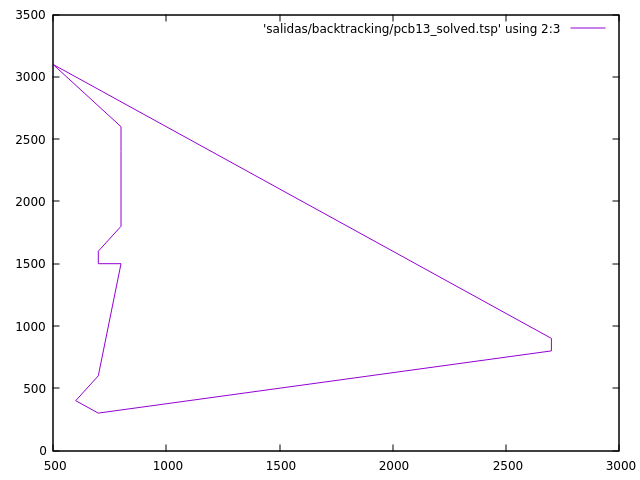
\includegraphics[width=70mm]{graficas/Backtracking/pcb13}}
  \subfigure[Brach and Bound. Peso = 8351]{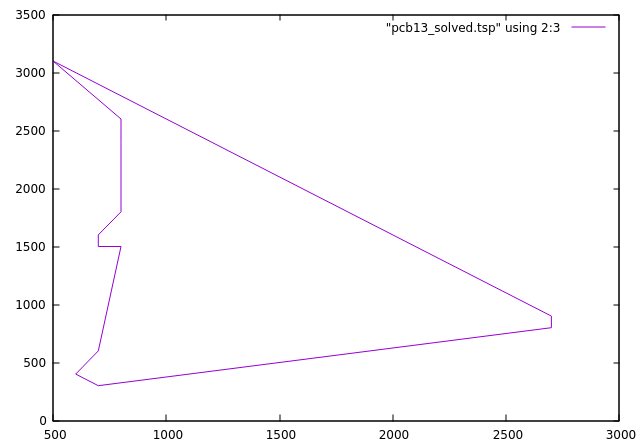
\includegraphics[width=70mm]{graficas/B&B/pcb13}}
\end{figure}

\newpage

\subsection{pr14}
\setcounter{subfigure}{0}

Branch and Bound:
\begin{itemize}
\item Nodos expandidos: 80852
\item Podas: 317840
\item Nº máximo de nodos vivos simultáneamente: 315823
\end{itemize}

\begin{figure}[H]
  \centering
  \subfigure[Greedy. Peso = 3565]{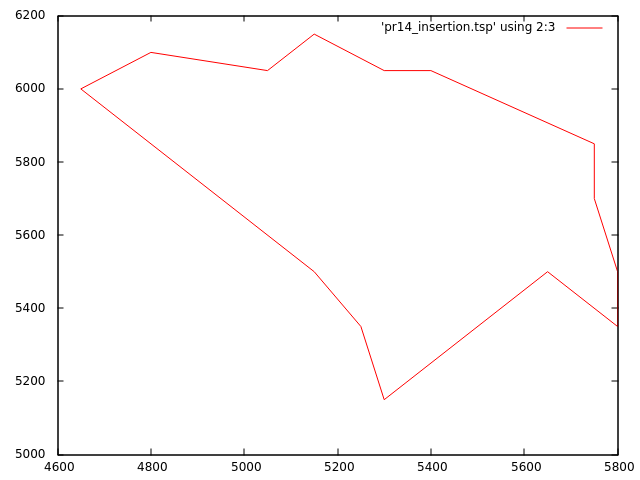
\includegraphics[width=70mm]{graficas/Greedy/pr14}}
  \subfigure[Backtracking. Peso = 3565]{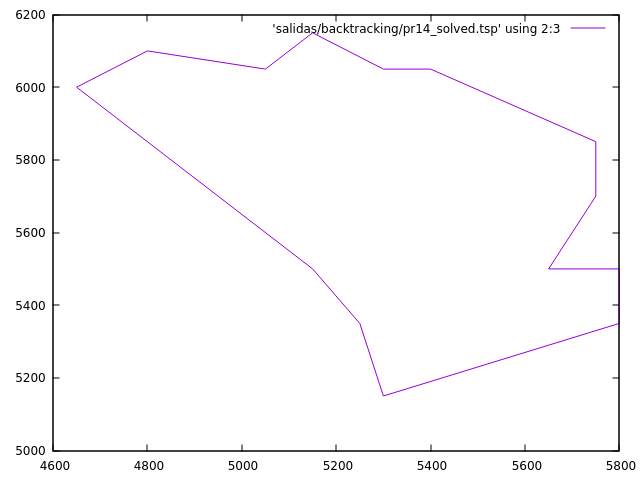
\includegraphics[width=70mm]{graficas/Backtracking/pr14}}
  \subfigure[Branch and Bound. Peso = 3565]{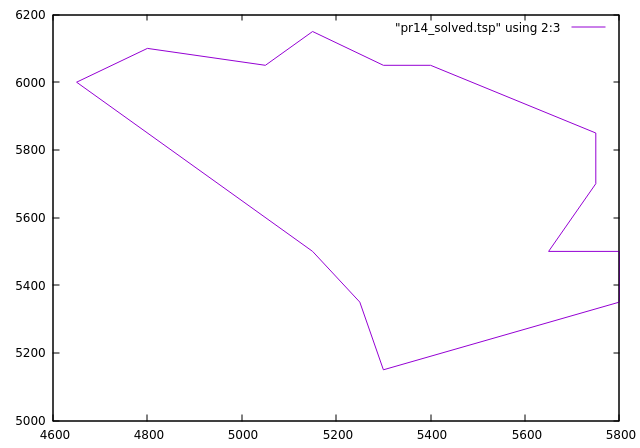
\includegraphics[width=70mm]{graficas/B&B/pr14}}
\end{figure}

\newpage

\subsection{pr15}
\setcounter{subfigure}{0}

Branch and Bound:
\begin{itemize}
\item Nodos expandidos: 131533
\item Podas: 547585
\item Nº máximo de nodos vivos simultáneamente: 546530
\end{itemize}

\begin{figure}[H]
  \centering
  \subfigure[Greedy. Peso = 3653]{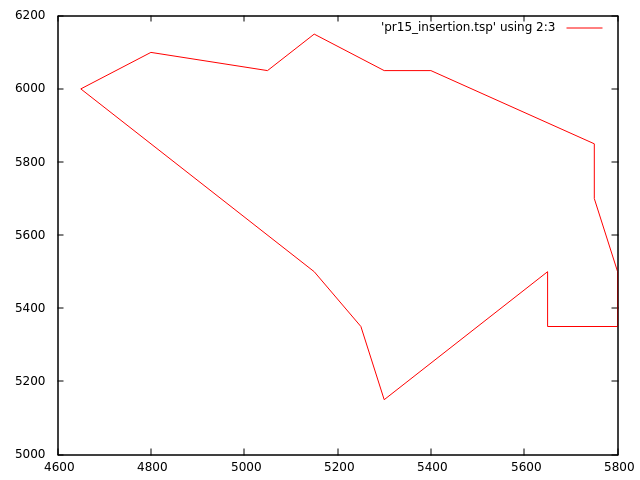
\includegraphics[width=70mm]{graficas/Greedy/pr15}}
  \subfigure[Backtracking. Peso = 3579]{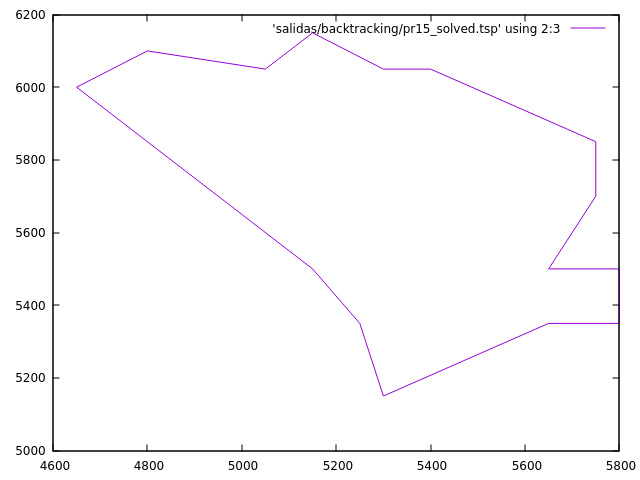
\includegraphics[width=70mm]{graficas/Backtracking/pr15}}
  \subfigure[Branch and Bound. Peso = 3579]{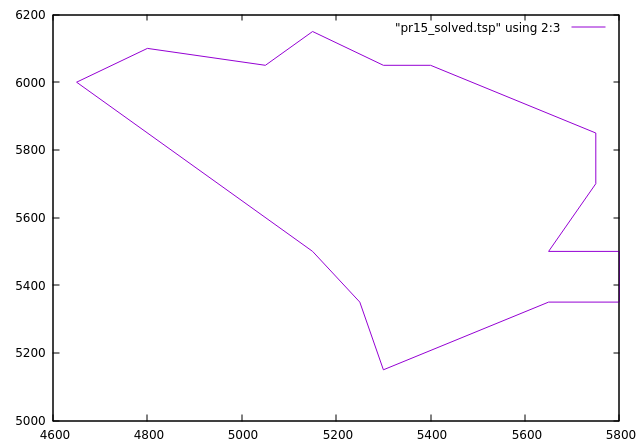
\includegraphics[width=70mm]{graficas/B&B/pr15}}
\end{figure}

\section{Conclusión}

Tras probar con los mismos datos tres algoritmos diferentes: Greedy,
Bactracking y Branch and Bound, podemos llegar a ciertas
conclusiones. Observamos que la ejecución más rápida se da con Greedy
y en la mayor parte de los casos encuentra la solución óptima al igual
que Backtracking y Branch and Bound. Con Backtracking y Branch and
Bound nos aseguramos llegar al camino hamiltoniano deseado (la
solución óptima) a cambio de una gran pérdida en eficiencia. Si
comparamos estos dos, B\&B llega a esta solución después que
Backtracking. Gracias a estas práctica hemos aprendido a realizar
nuestros propios algoritmos siguiendo las pautas dadas en clase y a
comparar la eficiencia de estos. Además hemos podido ver como en
ocasiones es preferible obtener una aproximación y no la solución
óptima a cambio de una mejora considerable en el tiempo de ejecución.

\end{document}
